\documentclass{beamer-control}
\usepackage{beamer-control-singlefile}
\INCLUDEONLY{Design Considerations}
\begin{document}
\CONCEPT{Design Considerations}

\begin{SUMMARY}
\begin{itemize}
\item Second-order systems
\item Higher-order systems
\end{itemize}
\vfill References:
\begin{itemize}
\item \astrom{§7.3}
\end{itemize}
\end{SUMMARY}



\SUBCONCEPT{Second-order systems}


\begin{frame}{Design considerations}
\begin{itemize}
\item The location of the eigenvalues of a system may be chosen with appropriate state feedback and these locations are the main design consideration
\item There is a trade-off between closed-loop performance, robustness of the system, and magnitude of control inputs
\item We examine these by studying second-order systems
\end{itemize}
\end{frame}


\begin{frame}{Second-order dynamics}
A general second-order system is given by the differential equation
\[\ddot{q}+2\zeta \omega_0 \dot{q}+\omega_0^2q=k\omega_0^2u, \quad y=q.\]
The state space representation is 
\[\frac{\mathrm{d} x}{\mathrm{d} t}=\begin{bmatrix}
	0 & \omega_0 \\
	-\omega_0 & -2 \zeta \omega_0
\end{bmatrix} x+\begin{bmatrix} 0 \\
k \omega_0 
\end{bmatrix}u, \quad y=\begin{bmatrix}
	1 & 0
\end{bmatrix} x,\]
where $x=\left(q,\tfrac{\dot{q}}{\omega_0}\right)$ is a normalised choice of states.\\
The parameter $\omega_0$ is known as the natural frequnecy of teh system and $\zeta$ is known as the damping ratio.
\end{frame}

\begin{frame}{Second-order dynamics}
The eigenvalues of this general system are 
\[\lambda=-\zeta \omega_0 \pm \omega_0 \sqrt{\zeta^2-1}.\]	
From this we can deduce that the system is stable if $\omega_0>0$ and $\zeta>0$. Also, the eigenvalues are complex if $\zeta>1$ and are real if $\zeta\leq 1$.\\

The parameter $\zeta$ describes systems that are
\begin{itemize}
	\item overdamped if $\zeta>1$ and exhibits exponentially decaying dynamics,
	\item critically damped if $\zeta=1$ and gives similarly decaying dynamics, 
	\item and is underamped if $0<\zeta < 1$ where the solutions are oscillatory with damped frequency $\omega_d=\omega_0\sqrt{1-\zeta^2}$.
\end{itemize}
\end{frame}

\begin{frame}{Second-order dynamics}
The simple form of second-order systems means we can derive analytical expressions for time and frequency responses.
\begin{figure}
	\centering
	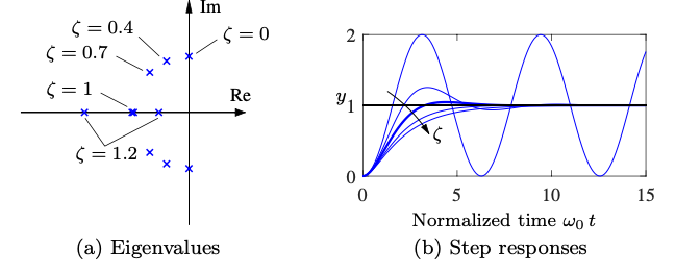
\includegraphics[width=0.5\linewidth]{figure7.8}
	\\
	\textbf{Figure 7.8:} Step response for a second-order system.
\end{figure}
\begin{figure}
	\centering
	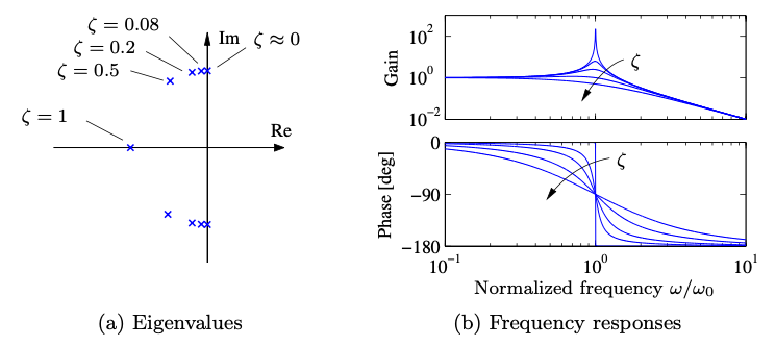
\includegraphics[width=0.5\linewidth]{figure7.9}
	\\
	\textbf{Figure 7.9:} Frequency response for a second-order system.
\end{figure}
\end{frame}


\begin{frame}{Second-order dynamics}
We can compute properties of the step response analytically as well

\begin{center}
	\begin{tabular}{|c|c|}
	\hline
	Property & Value\\ & \\
	\hline
	Steady-state value & $k$ \\  & \\
	Rise time & $T_r=\frac{e^\frac{\varphi}{\tan \varphi}}{\omega_0}$, where $\varphi=\arccos \zeta$ \\ & \\
	Overshoot & $M_p=e^{\frac{-\pi \zeta}{\sqrt{1-\zeta^2}}}$ \\ & \\
	2\% settling time & $T_s\approx \frac{4}{\zeta \omega_0}$
	\\
	\hline
\end{tabular}
\end{center}
\end{frame}


\SUBCONCEPT{Higher-order systems}

\begin{frame}{Dominant eigenvalues}
\begin{itemize}
\item Systems more complicated than second-order are characterised by the dominant eigenvalues
\item For stable systems, dominant eigenvalues are those that are closest to the imaginary axis as these correspond to the `slowest' response
\item By superposition, the faster dynamics corresponding to eigenvalues further from the imaginary axis will decay much quicker than the dominant terms
\item For eigenvalue assignment of higher-order systems, we therefore must consider how the dominant poles will affect the dynamics in closed-loop
\end{itemize}
\end{frame}


\SUMMARYFRAME
\FINALE

\end{document}
